\documentclass[tikz,border=8pt]{standalone}
\usepackage[T1]{fontenc}
\usepackage{lmodern}
\usepackage{amsmath,amssymb}
\usetikzlibrary{arrows.meta,positioning,shapes.geometric,fit,calc,backgrounds}

\definecolor{navy}{RGB}{20,45,90}
\definecolor{slate}{RGB}{60,85,125}
\definecolor{teal}{RGB}{0,115,115}
\definecolor{crimson}{RGB}{165,30,45}
\definecolor{amber}{RGB}{195,115,0}
\definecolor{softblue}{RGB}{238,244,252}
\definecolor{softteal}{RGB}{232,247,246}
\definecolor{softred}{RGB}{253,238,240}
\definecolor{softamber}{RGB}{254,247,232}

\begin{document}
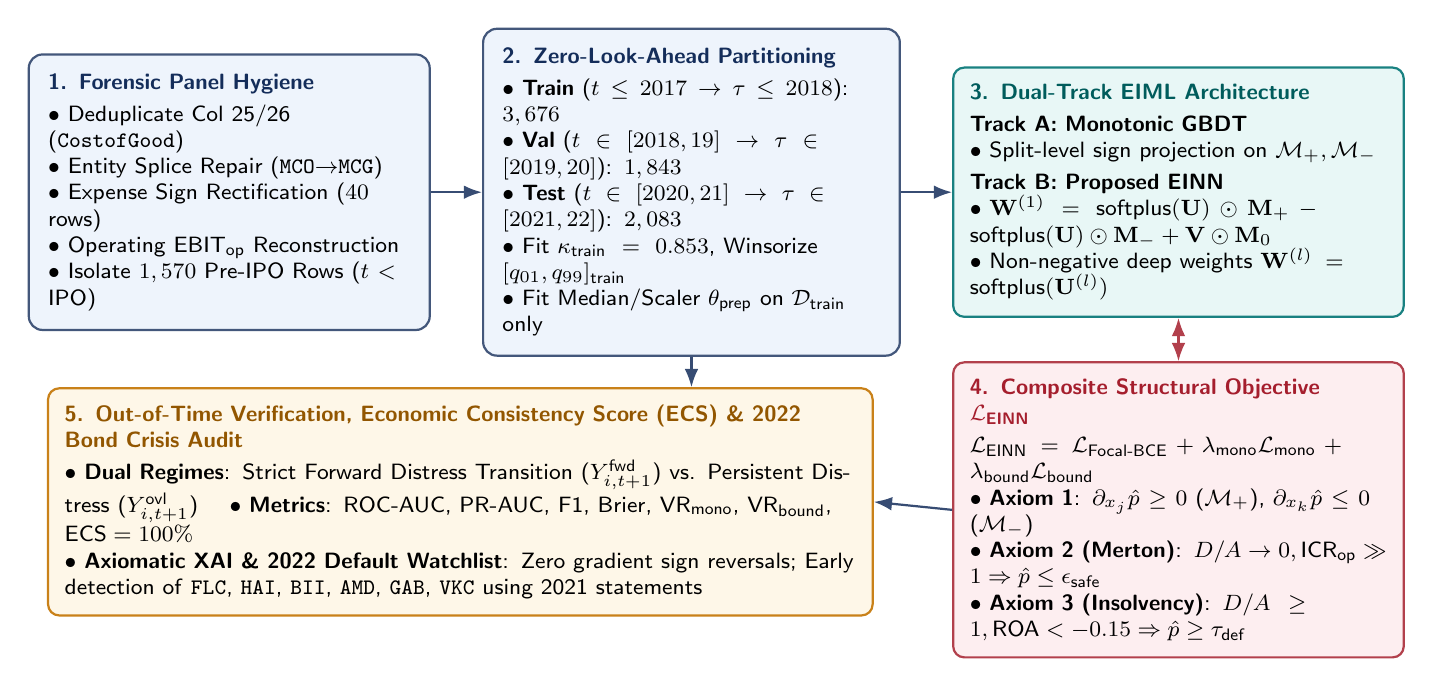
\begin{tikzpicture}[
    font=\sffamily\footnotesize,
    >=Latex,
    box/.style={draw=navy, thick, rounded corners=4pt, fill=white, align=center, inner sep=6pt},
    stage/.style={draw=navy!80, thick, rounded corners=5pt, fill=softblue, align=left, inner sep=7pt},
    lossbox/.style={draw=crimson!85, thick, rounded corners=4pt, fill=softred, align=left, inner sep=6pt},
    modelbox/.style={draw=teal!90, thick, rounded corners=4pt, fill=softteal, align=left, inner sep=6pt},
    evalbox/.style={draw=amber!90, thick, rounded corners=4pt, fill=softamber, align=left, inner sep=6pt},
    arrow/.style={->, thick, draw=navy!85}
]

% Stage 1: Forensic Hygiene
\node[stage, text width=4.6cm] (s1) at (0,0) {
    \textbf{\color{navy}1. Forensic Panel Hygiene}\\
    \vspace{2pt}
    $\bullet$ Deduplicate Col 25/26 (\texttt{CostofGood})\\
    $\bullet$ Entity Splice Repair (\texttt{MCO}$\to$\texttt{MCG})\\
    $\bullet$ Expense Sign Rectification ($40$ rows)\\
    $\bullet$ Operating $\text{EBIT}_{\text{op}}$ Reconstruction\\
    $\bullet$ Isolate $1,570$ Pre-IPO Rows ($t < \text{IPO}$)
};

% Stage 2: Strict Temporal Partitioning
\node[stage, text width=4.8cm, right=0.65cm of s1] (s2) {
    \textbf{\color{navy}2. Zero-Look-Ahead Partitioning}\\
    \vspace{2pt}
    $\bullet$ \textbf{Train} ($t \le 2017 \to \tau \le 2018$): $3,676$\\
    $\bullet$ \textbf{Val} ($t \in [2018,19] \to \tau \in [2019,20]$): $1,843$\\
    $\bullet$ \textbf{Test} ($t \in [2020,21] \to \tau \in [2021,22]$): $2,083$\\
    $\bullet$ Fit $\kappa_{\text{train}}=0.853$, Winsorize $[q_{01},q_{99}]_{\text{train}}$\\
    $\bullet$ Fit Median/Scaler $\theta_{\text{prep}}$ on $\mathcal{D}_{\text{train}}$ only
};

% Stage 3: Dual-Track EIML Architecture
\node[modelbox, text width=5.3cm, right=0.65cm of s2] (s3) {
    \textbf{\color{teal!80!black}3. Dual-Track EIML Architecture}\\
    \vspace{2pt}
    \textbf{Track A: Monotonic GBDT}\\
    $\bullet$ Split-level sign projection on $\mathcal{M}_+, \mathcal{M}_-$\\
    \vspace{2pt}
    \textbf{Track B: Proposed EINN}\\
    $\bullet$ $\mathbf{W}^{(1)} = \text{softplus}(\mathbf{U})\odot \mathbf{M}_+ - \text{softplus}(\mathbf{U})\odot \mathbf{M}_- + \mathbf{V}\odot \mathbf{M}_0$\\
    $\bullet$ Non-negative deep weights $\mathbf{W}^{(l)} = \text{softplus}(\mathbf{U}^{(l)})$
};

% Stage 4: Theory-Informed Regularization
\node[lossbox, text width=5.3cm, below=0.55cm of s3] (s4) {
    \textbf{\color{crimson}4. Composite Structural Objective $\mathcal{L}_{\text{EINN}}$}\\
    \vspace{2pt}
    $\mathcal{L}_{\text{EINN}} = \mathcal{L}_{\text{Focal-BCE}} + \lambda_{\text{mono}}\mathcal{L}_{\text{mono}} + \lambda_{\text{bound}}\mathcal{L}_{\text{bound}}$\\
    $\bullet$ \textbf{Axiom 1}: $\partial_{x_j}\hat{p} \ge 0$ ($\mathcal{M}_+$), $\partial_{x_k}\hat{p} \le 0$ ($\mathcal{M}_-$)\\
    $\bullet$ \textbf{Axiom 2 (Merton)}: $D/A \to 0, \text{ICR}_{\text{op}} \gg 1 \Rightarrow \hat{p} \le \epsilon_{\text{safe}}$\\
    $\bullet$ \textbf{Axiom 3 (Insolvency)}: $D/A \ge 1, \text{ROA} < -0.15 \Rightarrow \hat{p} \ge \tau_{\text{def}}$
};

% Stage 5: Audit & Early Warning Output
\node[evalbox, text width=10.05cm, below=0.55cm of $(s1.south)!0.5!(s2.south)$] (s5) {
    \textbf{\color{amber!75!black}5. Out-of-Time Verification, Economic Consistency Score (ECS) \& 2022 Bond Crisis Audit}\\
    \vspace{2pt}
    $\bullet$ \textbf{Dual Regimes}: Strict Forward Distress Transition ($Y_{i,t+1}^{\text{fwd}}$) vs. Persistent Distress ($Y_{i,t+1}^{\text{ovl}}$) \quad
    $\bullet$ \textbf{Metrics}: ROC-AUC, PR-AUC, F1, Brier, $\text{VR}_{\text{mono}}$, $\text{VR}_{\text{bound}}$, $\text{ECS} = 100\%$\\
    $\bullet$ \textbf{Axiomatic XAI \& 2022 Default Watchlist}: Zero gradient sign reversals; Early detection of \texttt{FLC}, \texttt{HAI}, \texttt{BII}, \texttt{AMD}, \texttt{GAB}, \texttt{VKC} using 2021 statements
};

\draw[arrow] (s1.east) -- (s2.west);
\draw[arrow] (s2.east) -- (s3.west);
\draw[arrow, <->, draw=crimson!85] (s3.south) -- (s4.north);
\draw[arrow] (s4.west) -- (s5.east);
\draw[arrow] (s2.south) -- (s2.south |- s5.north);

\end{tikzpicture}
\end{document}
